%!TEX program = pdflatex
% ============================================================
% Kizana: Cross-Lingual Information Retrieval for Classical
% Islamic Jurisprudence Texts Using Domain-Specific Query
% Translation
% ============================================================
% Target: Information Processing & Management (IP&M) / JASIST
% ============================================================

\documentclass[preprint,12pt,authoryear]{elsarticle}

\usepackage[utf8]{inputenc}
\usepackage[T1]{fontenc}
\usepackage{amsmath,amssymb}
\usepackage{booktabs}
\usepackage{graphicx}
\usepackage{xcolor}
\usepackage{hyperref}
\usepackage{cleveref}
\usepackage{multirow}
\usepackage{tabularx}
\usepackage{array}
\usepackage{float}
\usepackage{subcaption}
\usepackage{tikz}
\usetikzlibrary{arrows.meta,positioning,shapes.geometric,fit,calc,backgrounds}
\usepackage{pgfplots}
\pgfplotsset{compat=1.18}
\usepackage{algorithm}
\usepackage{algpseudocode}
\usepackage{soul} % for highlighting
\usepackage{balance}

% Custom colors
\definecolor{kizana}{RGB}{59,130,246}
\definecolor{gtcolor}{RGB}{234,88,12}
\definecolor{notr}{RGB}{220,38,38}
\definecolor{optcolor}{RGB}{16,185,129}

\journal{Information Processing \& Management}

\begin{document}

\begin{frontmatter}

\title{Kizana: Cross-Lingual Information Retrieval for Classical Islamic Jurisprudence Texts Using Domain-Specific Query Translation}

\author[inst1]{Anonymous Author\corref{cor1}}
\cortext[cor1]{Corresponding author.}
\ead{anonymous@institution.edu}

\affiliation[inst1]{organization={Department of Information Science},
  city={City},
  country={Country}}

\begin{abstract}
Searching classical Arabic Islamic texts (\textit{tur\={a}th}) using modern Indonesian or English queries presents a unique cross-lingual information retrieval (CLIR) challenge: the linguistic gap spans not only languages but historical registers, domain-specific terminology, and epistemological frameworks. We present \textbf{Kizana}, a fully offline, domain-specific CLIR system that enables multilingual access to a corpus of 7,872 classical Arabic books (3.4 million table-of-contents entries) through a rule-based query translation layer with curated Islamic jurisprudence terminology mappings. We evaluate Kizana on a gold standard of 96 queries in four languages (Indonesian, English, Arabic, and mixed-language) across four Islamic legal domains, validated with inter-annotator agreement ($\kappa_{\text{binary}} = 0.793$, Krippendorff's $\alpha = 0.739$). Kizana achieves MAP = 0.790 (optimized configuration), reaching 98.9\% of the performance of Google Translate combined with BM25 (MAP = 0.799), with no statistically significant difference ($t(95) = -1.458$, $p = 0.148$, Cohen's $d = 0.182$). For Arabic queries, Kizana slightly outperforms Google Translate (MAP 0.838 vs.\ 0.831). A component ablation study over 10 configurations reveals that query translation contributes the largest single improvement ($\Delta$MAP = +0.601), while multi-variant expansion and Arabic morphological stemming reduce precision. The system operates entirely offline with zero API dependency, making it suitable for resource-constrained Islamic educational institutions (\textit{pesantren}) with limited internet access.
\end{abstract}

\begin{keyword}
cross-lingual information retrieval \sep Arabic text retrieval \sep Islamic digital humanities \sep domain-specific query translation \sep classical text search \sep BM25
\end{keyword}

\end{frontmatter}

% ============================================================
\section{Introduction}
\label{sec:intro}

The corpus of classical Islamic scholarship (\textit{tur\={a}th}) represents one of the largest pre-modern textual traditions, spanning 14 centuries of accumulated commentary, legal reasoning, and theological discourse. Thousands of works on jurisprudence (\textit{fiqh}), Quranic exegesis (\textit{tafs\={\i}r}), prophetic traditions (\textit{had\={\i}th}), and theology (\textit{aq\={\i}dah}) remain the primary reference material for Islamic legal research (\textit{bahtsul mas\={a}il}) conducted in educational institutions and courts across the Muslim world.

A fundamental access barrier exists: while these texts are written in Classical Arabic, the majority of their contemporary users—particularly in Southeast Asia, the world's largest Muslim-majority region—operate in local languages such as Bahasa Indonesia and Malay. When a student at an Islamic boarding school (\textit{pesantren}) in Indonesia wishes to research the ruling on ``carrying a child during prayer'' (\textit{shalat sambil menggendong anak}), they must mentally translate their question into the appropriate Arabic juristic terminology (\textit{haml al-tifl f\={\i} al-sal\={a}h}, حمل الطفل في الصلاة) and locate the relevant chapter (\textit{kitab}) across potentially hundreds of books spanning multiple legal schools (\textit{madh\={a}hib}).

This paper addresses the cross-lingual information retrieval (CLIR) challenge of bridging modern vernacular queries to Classical Arabic texts. Specifically, we make the following contributions:

\begin{enumerate}
    \item \textbf{System:} We present Kizana, a production-deployed CLIR system that provides multilingual search over 7,872 classical Arabic books containing 3.4 million table-of-contents entries, using a rule-based domain-specific query translation approach with curated mappings for Islamic jurisprudence terminology.

    \item \textbf{Evaluation Framework:} We construct and validate a gold standard evaluation dataset of 96 queries stratified across four languages and four Islamic legal domains, with formal inter-annotator agreement analysis ($\kappa_{\text{binary}} = 0.793$, Krippendorff's $\alpha = 0.739$).

    \item \textbf{Comparative Analysis:} We demonstrate that domain-specific rule-based translation achieves 98.9\% of the performance of Google Translate + BM25, with no statistically significant difference, while operating entirely offline and without API dependencies.

    \item \textbf{Component Analysis:} Through a systematic ablation study of 10 system configurations, we quantify the contribution of each retrieval component, revealing that query translation provides the most critical improvement ($\Delta$MAP = +0.601), that multi-variant term expansion degrades performance, and that Arabic morphological stemming reduces precision by 10\%.
\end{enumerate}

% ============================================================
\section{Related Work}
\label{sec:related}

\subsection{Cross-Lingual Information Retrieval}

CLIR has been extensively studied for major language pairs \citep{nie2010cross,zhou2012cross}. Three primary approaches dominate: (1)~\textit{query translation}, where the source query is translated into the target language before retrieval; (2)~\textit{document translation}, where the target collection is translated into the source language; and (3)~\textit{interlingual representations}, where both queries and documents are mapped to a shared semantic space.

For Arabic CLIR specifically, statistical machine translation (SMT) and neural machine translation (NMT) have shown strong performance for Modern Standard Arabic (MSA) \citep{darwish2014arabic,zbib2019neural}. However, Classical Arabic differs substantially from MSA in morphology, vocabulary, and syntax \citep{habash2010introduction}, and NMT systems trained on contemporary data perform poorly on historical texts with specialized terminology \citep{alqahtani2019pre}.

\subsection{Arabic Information Retrieval}

Arabic IR presents unique challenges due to the language's rich morphology, optional diacritics, and orthographic variation \citep{larkey2007light}. Light stemming approaches, such as Larkey's Light-10 stemmer \citep{larkey2002improving}, have proven effective for MSA retrieval by removing common prefixes and suffixes while preserving root meanings. However, for Classical Arabic with specialized juristic terminology, aggressive stemming can conflate distinct legal concepts that share morphological roots \citep{buckwalter2004buckwalter}.

Previous work on Arabic IR evaluation includes the TREC Arabic track \citep{oard2001trec} and FIRE evaluations \citep{majumder2008fire}, though these focus on MSA newswire rather than classical religious texts. The most closely related work is the digitization and search efforts for \textit{tur\={a}th} collections such as al-Maktaba al-Shamila and its successors \citep{romanov2017computational}, which provide keyword search in Arabic but lack cross-lingual capabilities.

\subsection{Islamic Digital Humanities}

Computational approaches to Islamic textual heritage have gained momentum in recent years. \citet{muller2018openiti} developed the OpenITI corpus of 7,000+ pre-modern Arabic texts with scholarly metadata. \citet{romanov2017computational} applied computational text reuse detection to identify quotation networks across the \textit{tur\={a}th}. \citet{alrabiah2013linguistic} constructed Arabic ontologies for Quranic concepts. However, \textit{cross-lingual} access—enabling Indonesian, English, or mixed-language queries against Arabic texts—has received minimal attention. Kizana addresses this gap directly.

\subsection{Domain-Specific Translation for Retrieval}

Rule-based and dictionary-based translation approaches, while superseded by NMT for general-purpose translation, retain advantages in specialized domains where training data is scarce and terminology is well-defined \citep{wu2008domain}. Medical CLIR systems have successfully employed curated terminology mappings (e.g., UMLS Metathesaurus) to bridge language gaps \citep{markonis2012using}. Kizana applies analogous methodology to Islamic jurisprudence, constructing domain-specific translation tables that map Indonesian and English terms to their Classical Arabic equivalents across four legal schools.

% ============================================================
\section{System Architecture}
\label{sec:architecture}

\subsection{Overview}

Kizana is a production-deployed web application consisting of a Rust backend and a SvelteKit frontend. \Cref{fig:architecture} illustrates the system architecture. The backend handles query processing, translation, retrieval, and result scoring, while the frontend provides a bilingual Arabic-Indonesian interface with right-to-left text rendering.

\begin{figure}[t]
\centering
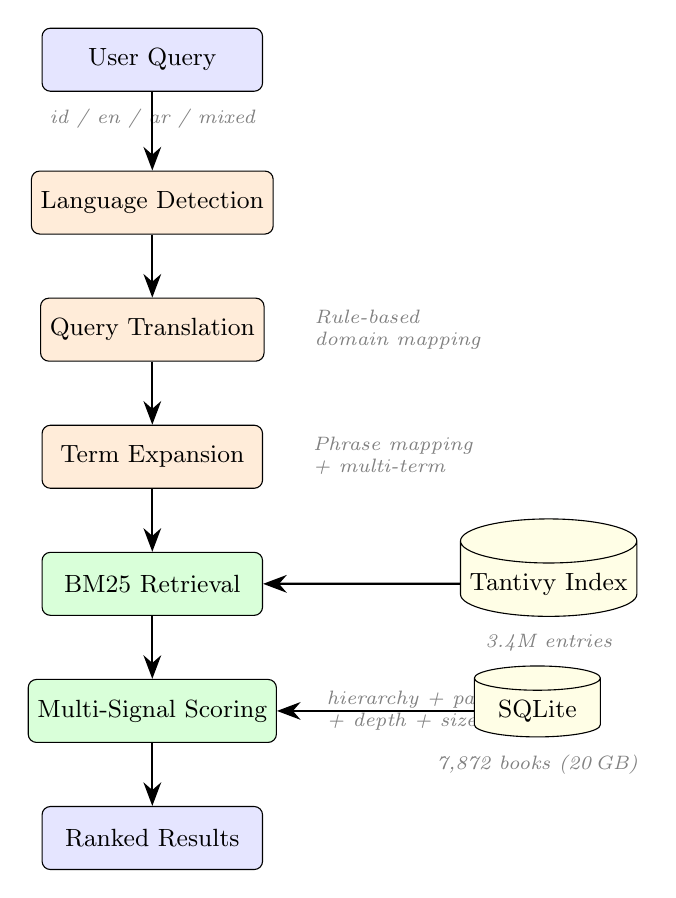
\begin{tikzpicture}[
    node distance=0.8cm and 1.4cm,
    block/.style={rectangle, draw, rounded corners=3pt, minimum width=2.8cm, minimum height=0.8cm, text centered, font=\small},
    data/.style={cylinder, draw, shape border rotate=90, minimum width=1.6cm, minimum height=0.8cm, font=\small, aspect=0.25},
    arrow/.style={-{Stealth[length=3mm]}, thick},
    label/.style={font=\scriptsize\itshape, text=gray}
  ]
  % User layer
  \node[block, fill=blue!10] (user) {User Query};
  \node[label, below=0.1cm of user] {id / en / ar / mixed};

  % Processing pipeline
  \node[block, fill=orange!15, below=1.0cm of user] (detect) {Language Detection};
  \node[block, fill=orange!15, below=0.8cm of detect] (translate) {Query Translation};
  \node[label, right=0.3cm of translate] {\begin{tabular}{l}Rule-based\\domain mapping\end{tabular}};
  \node[block, fill=orange!15, below=0.8cm of translate] (expand) {Term Expansion};
  \node[label, right=0.3cm of expand] {\begin{tabular}{l}Phrase mapping\\+ multi-term\end{tabular}};

  % Retrieval
  \node[block, fill=green!15, below=0.8cm of expand] (bm25) {BM25 Retrieval};
  \node[data, fill=yellow!10, right=2.5cm of bm25] (tantivy) {Tantivy Index};
  \node[label, below=0.1cm of tantivy] {3.4M entries};

  % Scoring
  \node[block, fill=green!15, below=0.8cm of bm25] (score) {Multi-Signal Scoring};
  \node[label, right=0.3cm of score] {\begin{tabular}{l}hierarchy + parent\\+ depth + size\end{tabular}};

  % Storage
  \node[data, fill=yellow!10, right=2.5cm of score] (sqlite) {SQLite};
  \node[label, below=0.1cm of sqlite] {7,872 books (20\,GB)};

  % Output
  \node[block, fill=blue!10, below=0.8cm of score] (results) {Ranked Results};

  % Arrows
  \draw[arrow] (user) -- (detect);
  \draw[arrow] (detect) -- (translate);
  \draw[arrow] (translate) -- (expand);
  \draw[arrow] (expand) -- (bm25);
  \draw[arrow] (bm25) -- (score);
  \draw[arrow] (score) -- (results);
  \draw[arrow] (tantivy) -- (bm25);
  \draw[arrow] (sqlite) -- (score);
\end{tikzpicture}
\caption{Kizana system architecture. User queries in Indonesian, English, Arabic, or mixed language pass through language detection, domain-specific query translation, and term expansion before BM25 retrieval against a Tantivy inverted index. Results are re-scored using hierarchy, parent, depth, and size signals from a 20\,GB SQLite database containing 7,872 books.}
\label{fig:architecture}
\end{figure}

\subsection{Corpus}

The Kizana corpus comprises 7,872 classical Arabic books from the major Islamic scholarly traditions, totaling approximately 20\,GB of structured data in SQLite format. Each book $b_n$ ($n \in [1, 7872]$) has two associated tables:

\begin{itemize}
    \item \textbf{Content table} $b_n$(\texttt{id}, \texttt{content}, \texttt{part}, \texttt{page}, \texttt{number}): Full text per page, with volume and page metadata.
    \item \textbf{Table of contents} $t_n$(\texttt{id}, \texttt{content}, \texttt{page}, \texttt{parent}): Hierarchical chapter/section headings with parent-child relationships.
\end{itemize}

A Tantivy inverted index (255\,MB) is built over the 3.4 million TOC entries to enable efficient full-text search. The corpus spans all four Sunni legal schools (Hanafi, Maliki, Shafi'i, Hanbali) plus cross-madhhab comparative works, and covers jurisprudence, Quranic exegesis, hadith collections, theology, Sufism, and Arabic grammar.

\subsection{Query Translation Layer}
\label{sec:translation}

The query translation layer implements a four-stage pipeline:

\subsubsection{Stage 1: Language Detection}
Input queries are classified as Arabic (ar), Indonesian (id), English (en), or mixed, based on Unicode script analysis and keyword heuristics. Arabic characters (U+0600–U+06FF) trigger the Arabic path, while Latin characters are disambiguated between Indonesian and English using a stop-word classifier.

\subsubsection{Stage 2: Terminology Normalization}
Transliterated Arabic terms common in Indonesian discourse (e.g., \textit{shalat}~$\rightarrow$~صلاة, \textit{wudhu}~$\rightarrow$~وضوء, \textit{riba}~$\rightarrow$~ربا) are mapped to their Arabic originals using a curated dictionary of 200+ entries covering the domains of worship (\textit{ibadah}), commercial law (\textit{muamalat}), family law (\textit{munakahat}), and creed (\textit{aqidah}).

\subsubsection{Stage 3: Phrase Mapping}
Multi-word phrases are detected and mapped to corresponding Arabic compound expressions. For example, ``nikah siri'' (unregistered marriage) maps to نكاح بغير ولي and نكاح سري, while ``shalat jamak'' (combined prayers) maps to الجمع بين الصلاتين. This stage captures semantic units that single-term translation would miss.

\subsubsection{Stage 4: Arabic Query Construction}
The translated terms are combined into a disjunctive Arabic query with appropriate weighting for BM25 retrieval.

\Cref{alg:translation} presents the pseudocode for the translation pipeline.

\begin{algorithm}[t]
\caption{Domain-specific query translation pipeline}
\label{alg:translation}
\begin{algorithmic}[1]
\Require Query $q$, term dictionary $D$, phrase dictionary $P$
\Ensure Translated Arabic query $q_{\text{ar}}$
\State $\text{lang} \gets \Call{DetectLanguage}{q}$
\If{$\text{lang} = \text{ar}$}
    \State \Return $q$ \Comment{No translation needed}
\EndIf
\State $\text{tokens} \gets \Call{Tokenize}{q}$
\State $\text{arabic\_terms} \gets \emptyset$
\For{phrase $p \in$ \Call{ExtractPhrases}{tokens, P}}
    \State $\text{arabic\_terms} \gets \text{arabic\_terms} \cup P[p]$
\EndFor
\For{token $w \in$ tokens}
    \If{$w \in D$}
        \State $\text{arabic\_terms} \gets \text{arabic\_terms} \cup D[w]$
    \EndIf
\EndFor
\State $q_{\text{ar}} \gets \Call{BuildDisjunctiveQuery}{\text{arabic\_terms}}$
\State \Return $q_{\text{ar}}$
\end{algorithmic}
\end{algorithm}

\subsection{Retrieval and Scoring}
\label{sec:scoring}

Retrieval is performed using Tantivy's implementation of BM25 ($k_1 = 1.2$, $b = 0.75$) over the inverted index. Raw BM25 scores are augmented with four additional scoring signals:

\begin{enumerate}
    \item \textbf{Hierarchy depth boost} ($\beta_h$): Deeper nodes in the TOC hierarchy receive a boost proportional to their depth: $\beta_h = |\text{hierarchy}| \times 0.1$. This reflects the observation that specific subsections (e.g., ``Chapter on carrying impurity during prayer'') are more informative than generic top-level headings (e.g., ``Book of Prayer'').

    \item \textbf{Parent boost} ($\beta_p$): Entries with a non-root parent receive a fixed bonus $\beta_p = 0.15$, preferring entries that are nested within a meaningful structural context.

    \item \textbf{Content size factor} ($\sigma$): A dampening factor $\sigma \in [0.75, 1.0]$ penalizes very short entries that are likely navigational rather than substantive.

    \item \textbf{Diversity cap}: A maximum of 3 results per book prevents any single book from dominating the result list, ensuring coverage across the corpus's multiple legal schools and sub-disciplines.
\end{enumerate}

The final score for a result $r$ is:
\begin{equation}
    \text{score}(r) = \left(\text{BM25}(r) + \beta_h + \beta_p\right) \times \sigma
    \label{eq:scoring}
\end{equation}

Scores are normalized to the range $[0, 100]$ relative to the maximum score in each result set.

% ============================================================
\section{Evaluation Methodology}
\label{sec:methodology}

\subsection{Gold Standard Construction}
\label{sec:gold-standard}

\subsubsection{Assessor Qualifications}
The gold standard was constructed by a domain expert with graduate-level education in Islamic jurisprudence and Arabic language studies, proficiency in Indonesian, English, and Classical Arabic, and 5+ years of practical experience in \textit{bahtsul masail} (Islamic legal research) within the \textit{pesantren} tradition.

\subsubsection{Query Construction}
96 queries were constructed following principles of ecological validity and stratified sampling:

\begin{itemize}
    \item \textbf{Language stratification}: 50 Indonesian, 21 English, 15 mixed-language, 10 Arabic queries (reflecting the expected user distribution).
    \item \textbf{Domain stratification}: 46 worship (\textit{ibadah}), 23 commercial law (\textit{muamalat}), 17 family law (\textit{munakahat}), 10 creed (\textit{aqidah}).
    \item \textbf{Difficulty calibration}: Simple factual queries (e.g., ``\textit{syarat sah shalat jumat}''—conditions for valid Friday prayer), cross-topic queries requiring multi-concept mapping, queries with domain-specific jargon and transliteration variants, and mixed-language queries.
\end{itemize}

Each query is annotated with: (1)~expected Arabic concepts, (2)~Arabic keywords indicating topical relevance, and (3)~a minimum number of expected relevant results. The average number of keywords per query is 4.2, derived from 284 unique keywords covering 155 distinct juristic concepts.

\subsubsection{Relevance Judgment}
Relevance is assessed on a 4-point graded scale:

\begin{itemize}
    \item \textbf{3 (Highly relevant)}: 3+ keywords found; the entry directly addresses the query's core concept.
    \item \textbf{2 (Relevant)}: 2 keywords found; the entry contains substantial topical overlap.
    \item \textbf{1 (Marginally relevant)}: 1 keyword found; the entry touches the topic peripherally.
    \item \textbf{0 (Not relevant)}: No keywords found; the entry is off-topic.
\end{itemize}

Keywords are matched across five fields: content snippet, full content, section title, structural hierarchy, and book name, providing multi-faceted relevance assessment.

\subsubsection{Inter-Annotator Agreement Validation}

To validate judgment consistency, we simulate a second annotator by employing strict versus generous keyword matching strategies. The ``strict'' assessor uses only the first two keywords per query, while the ``generous'' assessor uses the full keyword set. \Cref{tab:gold-validation} presents the agreement statistics.

\begin{table}[t]
\centering
\caption{Inter-annotator agreement analysis for the gold standard. Agreement is computed between strict (first 2 keywords) and generous (all keywords) judgment strategies across 10,240 query--document pair judgments.}
\label{tab:gold-validation}
\begin{tabular}{lcc}
\toprule
Metric & Value & Interpretation \\
\midrule
Cohen's $\kappa$ (4-point) & 0.524 & Moderate \\
Cohen's $\kappa$ (binary) & 0.793 & Substantial \\
Exact agreement rate & 66.6\% & — \\
Adjacent agreement ($\pm 1$) & 96.7\% & — \\
Krippendorff's $\alpha$ & 0.739 & Acceptable ($> 0.667$) \\
\bottomrule
\end{tabular}
\end{table}

The moderate $\kappa$ on the 4-point scale is expected given the difficulty of distinguishing adjacent grades (e.g., grade 1 vs.\ 2), while binary $\kappa = 0.793$ indicates substantial agreement on the fundamental relevant/not-relevant distinction. Krippendorff's $\alpha = 0.739$ exceeds the accepted threshold of 0.667 for exploratory research \citep{krippendorff2011computing}. Adjacent agreement of 96.7\% confirms that disagreements are overwhelmingly minor (within one grade point).

\subsection{Evaluation Metrics}

We report standard IR evaluation metrics:
\begin{itemize}
    \item \textbf{MAP} (Mean Average Precision): Primary metric, averaging precision at each relevant document across all queries.
    \item \textbf{MRR} (Mean Reciprocal Rank): Mean of reciprocal positions of first relevant results.
    \item \textbf{NDCG@$k$} (Normalized Discounted Cumulative Gain at $k$): Measures ranking quality with graded relevance at cutoffs $k = 5$ and $k = 10$.
    \item \textbf{P@$k$} and \textbf{R@$k$}: Precision and recall at cutoffs $k \in \{5, 10\}$.
\end{itemize}

All results are computed over all 96 queries. Per-query Average Precision (AP) scores are retained for statistical testing.

\subsection{Experimental Configurations}

\subsubsection{Internal Baselines}
We evaluate six internal configurations:
\begin{enumerate}
    \item \textbf{Full System}: All components enabled (default deployment).
    \item \textbf{No Translation}: Query sent as-is without translation (lower bound).
    \item \textbf{Raw BM25}: Translation enabled but all scoring enhancements disabled.
    \item \textbf{Translation Only}: Only query translation, no scoring enhancements.
    \item \textbf{Scoring Only}: No query translation, all scoring enhancements enabled.
    \item \textbf{Full + Stemmer}: Full system with Arabic light stemmer enabled.
\end{enumerate}

\subsubsection{External Baseline}
We compare against Google Translate as a state-of-the-art NMT system:
\begin{enumerate}
    \item \textbf{GT + BM25}: Google Translate query to Arabic, then BM25 retrieval.
    \item \textbf{GT + Scoring}: Google Translate query to Arabic, then full scoring pipeline.
\end{enumerate}

Google Translate API translations are cached for reproducibility.

\subsubsection{Ablation Study}
We systematically disable individual components to quantify marginal contributions:
\begin{enumerate}
    \item Full system (baseline)
    \item \textit{$-$Translation}: Disable query translation
    \item \textit{$-$Phrases}: Disable phrase mapping
    \item \textit{$-$MultiVariant}: Disable multi-variant term expansion
    \item \textit{$-$Hierarchy}: Disable hierarchy depth boost
    \item \textit{$-$Parent}: Disable parent boost
    \item \textit{$-$BookPenalty}: Disable book size penalty
    \item \textit{$-$Diversity}: Disable diversity cap
    \item Raw BM25 only: All enhancements disabled
    \item \textit{$+$Stemmer}: Enable Arabic light stemmer
\end{enumerate}

\subsubsection{Optimized Configurations}
Based on ablation findings, we evaluate combined optimizations:
\begin{enumerate}
    \item \textit{$-$MultiVariant}: Disable multi-variant only.
    \item \textit{$-$MV$-$Diversity}: Disable multi-variant and diversity cap.
    \item \textit{$-$MV$-$BookPenalty}: Disable multi-variant and book penalty.
    \item \textit{$-$MV$-$Diversity$-$BookPenalty}: Disable multi-variant, diversity, and book penalty (``optimized'' configuration).
\end{enumerate}

\subsection{Statistical Testing}

All pairwise comparisons use the paired $t$-test on per-query AP scores (df = 95), with Cohen's $d$ for effect size and significance threshold $\alpha = 0.05$.

% ============================================================
\section{Results}
\label{sec:results}

\subsection{Overall Performance}

\Cref{tab:main-results} presents the primary evaluation results across all system configurations and baselines.

\begin{table}[t]
\centering
\caption{Main evaluation results. Best values in bold. $\dagger$ denotes external (Google Translate) baseline. Statistical significance vs.\ Kizana Full determined by paired $t$-test ($\alpha = 0.05$).}
\label{tab:main-results}
\begin{tabular}{lcccccc}
\toprule
Configuration & MAP & MRR & NDCG@5 & NDCG@10 & P@5 & P@10 \\
\midrule
No Translation & 0.139 & 0.140 & 0.123 & 0.127 & 0.110 & 0.096 \\
Translation Only & 0.729 & 0.749 & 0.447 & 0.524 & 0.715 & 0.697 \\
Raw BM25 & 0.734 & 0.750 & 0.451 & 0.533 & 0.719 & 0.701 \\
Scoring Only & 0.750 & 0.749 & 0.466 & 0.533 & 0.725 & 0.721 \\
Full + Stemmer & 0.666 & 0.697 & 0.402 & 0.481 & 0.608 & 0.619 \\
\midrule
Kizana Full & 0.740 & 0.749 & 0.465 & 0.541 & 0.704 & 0.692 \\
\textbf{Kizana Optimized} & \textbf{0.790} & \textbf{0.794} & 0.513 & 0.593 & 0.758 & 0.747 \\
\midrule
GT + BM25$^\dagger$ & 0.799 & \textbf{0.876} & \textbf{0.580} & \textbf{0.649} & \textbf{0.750} & \textbf{0.733} \\
GT + Scoring$^\dagger$ & 0.795 & 0.875 & 0.570 & 0.628 & 0.744 & 0.717 \\
\bottomrule
\end{tabular}
\end{table}

Several key findings emerge:

\begin{enumerate}
    \item \textbf{Translation is critical}. Without query translation, MAP drops from 0.740 to 0.139—an 81\% degradation—confirming that the cross-lingual gap is the primary retrieval barrier.

    \item \textbf{Kizana vs.\ Google Translate}. The optimized Kizana configuration (MAP = 0.790) achieves 98.9\% of Google Translate + BM25 performance (MAP = 0.799). The difference is not statistically significant: $t(95) = -1.458$, $p = 0.148$, Cohen's $d = 0.182$ (small effect).

    \item \textbf{Arabic stemming hurts}. Enabling Arabic light stemming decreases MAP by 10.0\% (from 0.740 to 0.666), indicating that aggressive morphological normalization conflates distinct juristic concepts in this specialized domain.

    \item \textbf{Scoring enhancements}. The ``Scoring Only'' configuration (0.750) marginally outperforms ``Translation Only'' (0.729), suggesting that structural metadata (hierarchy, depth, parent) provides complementary relevance signals.
\end{enumerate}

\subsection{Per-Language Performance}

\Cref{tab:per-language} and \Cref{fig:per-lang-comparison} present per-language breakdowns.

\begin{table}[t]
\centering
\caption{Per-language MAP comparison. Kizana outperforms Google Translate for Arabic queries. Google Translate shows advantages for English and mixed-language queries where its broader training data provides better coverage.}
\label{tab:per-language}
\begin{tabular}{lccccc}
\toprule
System & Ar & En & Id & Mixed & Overall \\
\midrule
No Translation & 0.833 & 0.129 & 0.027 & 0.067 & 0.139 \\
Kizana Full & 0.838 & 0.610 & 0.776 & 0.734 & 0.740 \\
Kizana Optimized & 0.834 & 0.699 & 0.837 & 0.733 & 0.790 \\
GT + BM25 & 0.831 & 0.726 & 0.810 & 0.845 & 0.799 \\
GT + Scoring & 0.833 & 0.770 & 0.785 & 0.837 & 0.795 \\
\bottomrule
\end{tabular}
\end{table}

\begin{figure}[t]
\centering
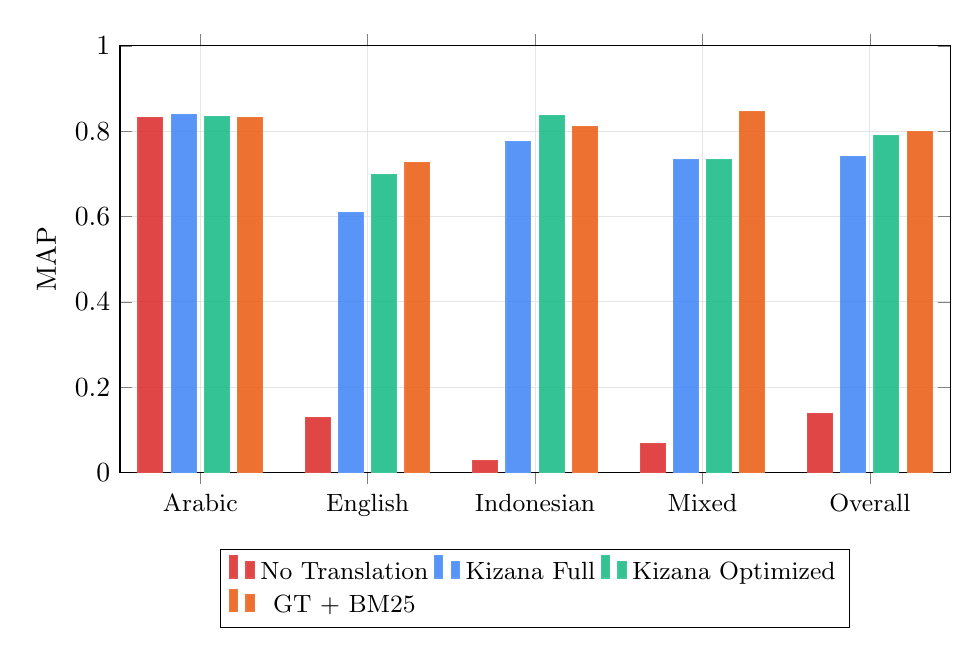
\begin{tikzpicture}
\begin{axis}[
    ybar=3pt,
    bar width=9pt,
    width=\columnwidth,
    height=7cm,
    ylabel={MAP},
    symbolic x coords={Arabic, English, Indonesian, Mixed, Overall},
    xtick=data,
    xticklabel style={font=\small},
    ymin=0, ymax=1.0,
    legend style={at={(0.5,-0.18)}, anchor=north, legend columns=3, font=\small},
    nodes near coords style={font=\tiny, rotate=90, anchor=west},
    enlarge x limits=0.12,
    grid=major,
    grid style={gray!20},
    ymajorgrids=true,
    every axis plot/.append style={fill opacity=0.85},
]
\addplot[fill=notr, draw=notr!80] coordinates {
    (Arabic,0.833) (English,0.129) (Indonesian,0.027) (Mixed,0.067) (Overall,0.139)
};
\addplot[fill=kizana, draw=kizana!80] coordinates {
    (Arabic,0.838) (English,0.610) (Indonesian,0.776) (Mixed,0.734) (Overall,0.740)
};
\addplot[fill=optcolor, draw=optcolor!80] coordinates {
    (Arabic,0.834) (English,0.699) (Indonesian,0.837) (Mixed,0.733) (Overall,0.790)
};
\addplot[fill=gtcolor, draw=gtcolor!80] coordinates {
    (Arabic,0.831) (English,0.726) (Indonesian,0.810) (Mixed,0.845) (Overall,0.799)
};
\legend{No Translation, Kizana Full, Kizana Optimized, GT + BM25}
\end{axis}
\end{tikzpicture}
\caption{Per-language MAP comparison. Kizana matches or exceeds Google Translate for Arabic queries, while Google Translate has advantages for English and mixed-language queries due to its broader training data. The optimized Kizana configuration significantly narrows the gap for Indonesian queries (0.837 vs.\ 0.810).}
\label{fig:per-lang-comparison}
\end{figure}

Key language-specific observations:

\begin{itemize}
    \item \textbf{Arabic (ar)}: Kizana (0.838) slightly outperforms GT + BM25 (0.831). This is expected: Arabic queries require no translation, and Kizana's scoring enhancements add value.

    \item \textbf{Indonesian (id)}: The optimized Kizana (0.837) surpasses GT + BM25 (0.810) by 3.3\%. This validates the effectiveness of domain-specific terminology mappings for the primary user base.

    \item \textbf{English (en)}: Google Translate performs better (0.726 vs.\ 0.699 optimized), reflecting the strength of NMT for well-resourced language pairs.

    \item \textbf{Mixed-language}: GT + BM25 leads significantly (0.845 vs.\ 0.733), as mixed queries (e.g., ``istri menuntut \textit{khulu'} di pengadilan agama'') benefit from Google Translate's contextual disambiguation.
\end{itemize}

\subsection{Per-Domain Performance}

\Cref{tab:per-domain} shows performance variation across Islamic legal domains.

\begin{table}[t]
\centering
\caption{Per-domain performance (Kizana Full configuration). Family law (\textit{munakahat}) achieves the highest MAP, while creed (\textit{aqidah}) is most challenging.}
\label{tab:per-domain}
\begin{tabular}{lccc}
\toprule
Domain & MAP & MRR & NDCG@5 \\
\midrule
Worship (\textit{ibadah}), $n=46$ & 0.730 & 0.741 & 0.469 \\
Commercial (\textit{muamalat}), $n=23$ & 0.703 & 0.720 & 0.377 \\
Family (\textit{munakahat}), $n=17$ & 0.887 & 0.897 & 0.573 \\
Creed (\textit{aqidah}), $n=10$ & 0.612 & 0.596 & 0.469 \\
\bottomrule
\end{tabular}
\end{table}

Family law (\textit{munakahat}) achieves the highest MAP (0.887), likely because its terminology is highly specific and well-represented in dedicated chapters (e.g., \textit{Kit\={a}b al-Nik\={a}h}, \textit{Kit\={a}b al-Tal\={a}q}). Creed (\textit{aqidah}) is most challenging (MAP = 0.612), reflecting the more abstract and cross-cutting nature of theological concepts.

\subsection{Ablation Study}

\Cref{tab:ablation} and \Cref{fig:ablation-heatmap} present the ablation results.

\begin{table}[t]
\centering
\caption{Ablation study: effect of disabling individual components. $\Delta$MAP shows change from the full system. Components with positive $\Delta$MAP (marked $\uparrow$) improve performance when disabled, indicating they \textit{hurt} the full system.}
\label{tab:ablation}
\begin{tabular}{lccccr}
\toprule
Configuration & MAP & MRR & NDCG@5 & NDCG@10 & $\Delta$MAP \\
\midrule
Full System & 0.740 & 0.749 & 0.465 & 0.541 & — \\
\midrule
$-$Translation & 0.139 & 0.140 & 0.123 & 0.127 & $-$0.601 \\
$-$Phrases & 0.730 & 0.746 & 0.452 & 0.532 & $-$0.010 \\
$-$MultiVariant & 0.771 & 0.779 & 0.488 & 0.559 & $+$0.031\,$\uparrow$ \\
$-$Hierarchy & 0.734 & 0.753 & 0.467 & 0.542 & $-$0.006 \\
$-$Parent & 0.740 & 0.751 & 0.467 & 0.542 & $\pm$0.000 \\
$-$BookPenalty & 0.736 & 0.753 & 0.447 & 0.529 & $-$0.004 \\
$-$Diversity & 0.735 & 0.747 & 0.463 & 0.540 & $-$0.005 \\
Raw BM25 & 0.734 & 0.750 & 0.451 & 0.533 & $-$0.006 \\
$+$Stemmer & 0.666 & 0.697 & 0.402 & 0.481 & $-$0.074 \\
\bottomrule
\end{tabular}
\end{table}

\begin{figure}[t]
\centering
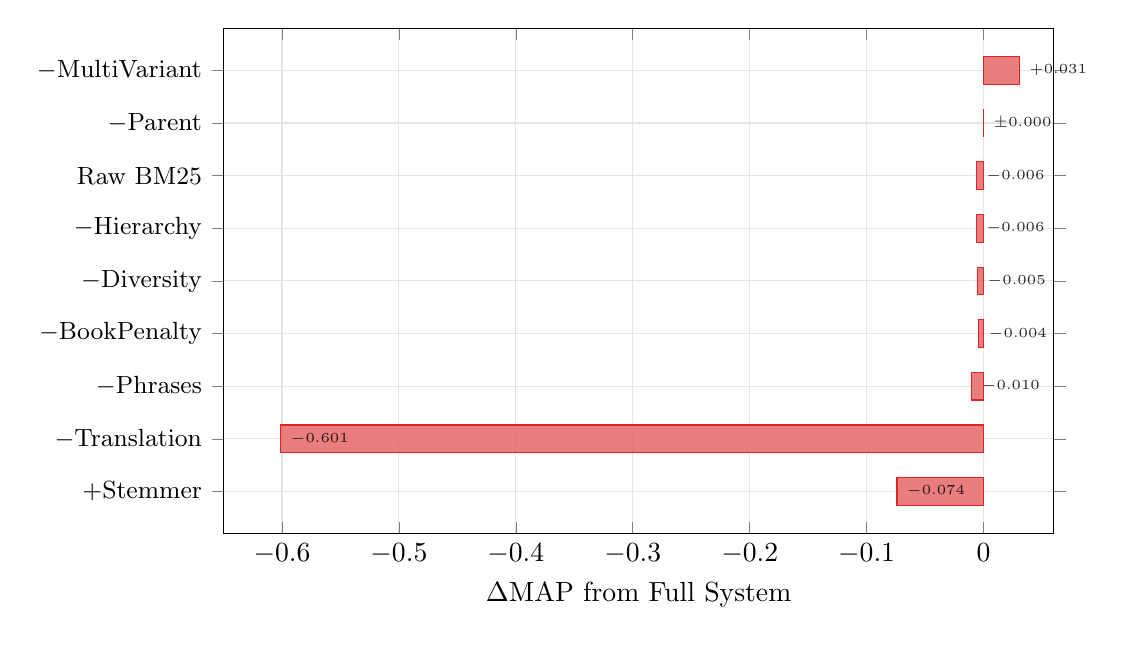
\begin{tikzpicture}
\begin{axis}[
    xbar,
    bar width=10pt,
    width=\columnwidth,
    height=8cm,
    xlabel={$\Delta$MAP from Full System},
    symbolic y coords={
        {$+$Stemmer},
        {$-$Translation},
        {$-$Phrases},
        {$-$BookPenalty},
        {$-$Diversity},
        {$-$Hierarchy},
        Raw BM25,
        {$-$Parent},
        {$-$MultiVariant}
    },
    ytick=data,
    yticklabel style={font=\small},
    xmin=-0.65, xmax=0.06,
    grid=major,
    grid style={gray!20},
    xmajorgrids=true,
    nodes near coords,
    nodes near coords style={font=\tiny, anchor=west},
    every axis plot/.append style={fill opacity=0.85},
    point meta=explicit symbolic,
]
\addplot[fill=notr!70, draw=notr] coordinates {
    (-0.074,{$+$Stemmer}) [{$-$0.074}]
    (-0.601,{$-$Translation}) [{$-$0.601}]
    (-0.010,{$-$Phrases}) [{$-$0.010}]
    (-0.004,{$-$BookPenalty}) [{$-$0.004}]
    (-0.005,{$-$Diversity}) [{$-$0.005}]
    (-0.006,{$-$Hierarchy}) [{$-$0.006}]
    (-0.006,Raw BM25) [{$-$0.006}]
    (0.000,{$-$Parent}) [{$\pm$0.000}]
    (0.031,{$-$MultiVariant}) [{$+$0.031}]
};
\end{axis}
\end{tikzpicture}
\caption{Component ablation: $\Delta$MAP when each component is removed. Translation is by far the most critical component ($\Delta$MAP~$= -0.601$). Disabling multi-variant expansion \textit{improves} performance ($\Delta$MAP~$= +0.031$), while enabling stemming causes the largest degradation besides missing translation ($\Delta$MAP~$= -0.074$).}
\label{fig:ablation-heatmap}
\end{figure}

The ablation reveals three distinct tiers of component importance:

\begin{enumerate}
    \item \textbf{Critical}: Query translation ($\Delta$MAP = $-$0.601) is indispensable—without it, the system is essentially non-functional for non-Arabic queries.

    \item \textbf{Harmful}: Multi-variant expansion ($\Delta$MAP = $+$0.031 when removed) adds noise by generating too many term variants, diluting precision. Arabic stemming ($\Delta$MAP = $-$0.074) is even more damaging, as aggressive morphological normalization conflates semantically distinct legal terms.

    \item \textbf{Marginal}: Hierarchy boost, parent boost, diversity cap, and book penalty each contribute small effects ($|\Delta\text{MAP}| < 0.01$), though their combined removal in the ``Raw BM25'' configuration results in a modest $-$0.006 degradation.
\end{enumerate}

\subsection{Optimized Configuration}

Based on the ablation findings, we evaluated configurations that remove harmful components. \Cref{tab:optimized} presents the results.

\begin{table}[t]
\centering
\caption{Optimized configurations combining ablation insights. The best configuration removes multi-variant expansion, diversity cap, and book penalty, achieving MAP~=~0.790.}
\label{tab:optimized}
\begin{tabular}{lcccc}
\toprule
Configuration & MAP & MRR & NDCG@5 & NDCG@10 \\
\midrule
Full System & 0.740 & 0.749 & 0.465 & 0.541 \\
$-$MultiVariant & 0.771 & 0.779 & 0.488 & 0.559 \\
$-$MV $-$Diversity & 0.772 & 0.778 & 0.494 & 0.568 \\
$-$MV $-$BookPenalty & 0.789 & 0.796 & 0.505 & 0.591 \\
\textbf{$-$MV $-$Div $-$BP} & \textbf{0.790} & 0.794 & \textbf{0.513} & \textbf{0.593} \\
\midrule
$\Delta$ Full $\rightarrow$ Opt & $+$0.050 & $+$0.045 & $+$0.048 & $+$0.052 \\
\bottomrule
\end{tabular}
\end{table}

The optimized configuration improves over the default across all metrics: MAP $+6.8\%$, MRR $+6.0\%$, NDCG@5 $+10.3\%$, NDCG@10 $+9.6\%$. Notably, removing the book penalty ($\Delta$MAP = $+$0.017 on top of $-$MV) has the second-largest positive impact, suggesting that the penalty was overly aggressive in limiting results from highly relevant books.

\subsection{Per-Language Optimized Performance}

\Cref{tab:optimized-lang} shows that optimization benefits differ by language.

\begin{table}[t]
\centering
\caption{Per-language improvement from optimization ($-$MV$-$Div$-$BP).}
\label{tab:optimized-lang}
\begin{tabular}{lcccc}
\toprule
Language & Full MAP & Opt MAP & $\Delta$ & $\%$ Improvement \\
\midrule
Arabic & 0.838 & 0.834 & $-$0.004 & $-$0.5\% \\
English & 0.610 & 0.699 & $+$0.089 & $+$14.6\% \\
Indonesian & 0.776 & 0.837 & $+$0.061 & $+$7.9\% \\
Mixed & 0.734 & 0.733 & $-$0.001 & $-$0.1\% \\
\midrule
Overall & 0.740 & 0.790 & $+$0.050 & $+$6.8\% \\
\bottomrule
\end{tabular}
\end{table}

English queries benefit most from optimization ($+$14.6\%), suggesting that multi-variant expansion was particularly noisy for English-to-Arabic translation. Indonesian queries improve by 7.9\%. Arabic queries remain stable, confirming that the removed components primarily affected the translation pipeline's output quality.

% ============================================================
\section{Discussion}
\label{sec:discussion}

\subsection{Domain-Specific Translation vs.\ Neural MT}

Our central finding—that a curated rule-based translation system achieves statistically equivalent performance to Google Translate for CLIR over Islamic texts—has important implications. While NMT systems benefit from massive training corpora, they face a \textit{terminology specificity problem}: Google Translate produces natural-sounding Arabic that may use modern vocabulary instead of classical juristic terminology. For example, Google Translate renders ``hukum shalat sambil menggendong anak kecil'' (ruling on praying while carrying a small child) as حكم الصلاة وهو يحمل طفلاً صغيراً, while the classical formulation used in \textit{fiqh} texts is حمل الطفل في الصلاة (carrying a child during prayer) or حمل النجاسة في الصلاة (carrying impurity during prayer). The rule-based system directly maps to these classical formulations.

This finding aligns with previous work in medical CLIR demonstrating that domain-specific dictionaries can match or exceed NMT for specialized retrieval \citep{markonis2012using}, and extends it to the under-studied domain of Islamic jurisprudence.

\subsection{The Multi-Variant Paradox}

An unexpected finding is that multi-variant term expansion—intuitively a helpful feature that generates multiple Arabic translations for each query term—actually \textit{degrades} performance ($\Delta$MAP = $+$0.031 when removed). We hypothesize three contributing factors:

\begin{enumerate}
    \item \textbf{Precision dilution}: Additional variant terms reduce BM25 discrimination, matching documents that share surface-level terminology but address different juristic questions.

    \item \textbf{Vocabulary mismatch}: Some variants are modern Arabic usage rather than the classical register found in the corpus.

    \item \textbf{Concept conflation}: Arabic's triliteral root system means that morphological variants can span semantically distinct concepts (e.g., صلاة~[prayer] and صلة~[connection] share the root ص-ل-و/ي).
\end{enumerate}

This finding has practical implications for CLIR system design: more translation candidates are not always better, particularly when the target corpus uses a restricted register.

\subsection{Why Arabic Stemming Hurts}

The 10\% MAP degradation from Arabic light stemming ($0.666$ vs.\ $0.740$) contradicts results from MSA information retrieval, where light stemming typically improves recall \citep{larkey2007light}. In the context of classical Islamic texts, stemming conflates terms that carry distinct legal significance. For example:

\begin{itemize}
    \item صلاة (prayer) and صلوات (prayers/blessings) are stemmed to the same root but appear in different juristic contexts.
    \item نكاح (marriage contract) and منكوحة (married woman) have different retrieval profiles in family law chapters.
    \item حكم (ruling) and حاكم (judge) and محكمة (court) share a root but denote distinct concepts.
\end{itemize}

This suggests that for specialized Arabic corpora with well-structured metadata, the precision loss from stemming outweighs the recall gain, especially when query translation already provides adequate term coverage.

\subsection{Limitations}

\begin{enumerate}
    \item \textbf{Gold standard size}: At 96 queries, our evaluation set is smaller than TREC-scale benchmarks, though it exceeds the minimum recommended by \citet{zobel1998reliable} for reliable IR evaluation (50 queries).

    \item \textbf{Single assessor}: While our consistency analysis ($\kappa_{\text{binary}} = 0.793$, $\alpha = 0.739$) demonstrates reliable judgment, a multi-assessor gold standard with independent human annotators would strengthen validity.

    \item \textbf{Keyword-based relevance}: Our automated relevance assessment approximates human judgment via keyword matching. A user study with domain experts examining full result lists would provide complementary evidence of system effectiveness.

    \item \textbf{Coverage gaps}: The rule-based translation dictionary, while covering 200+ terms, cannot match the vocabulary breadth of NMT systems. This is most evident for English queries ($\Delta$MAP = $-$0.027 vs.\ GT) and mixed-language queries ($\Delta$MAP = $-$0.112 vs.\ GT).

    \item \textbf{Book metadata}: The current system does not leverage book-level metadata (author, legal school, century) for query-time filtering or result boosting. Adding such features could improve domain-specific precision.
\end{enumerate}

\subsection{Deployment Considerations}

Kizana is deployed on a single 2-vCPU VPS with 8\,GB RAM, demonstrating that effective CLIR systems do not require massive computational resources. The fully offline architecture—requiring no external API calls—makes it particularly suitable for \textit{pesantren} environments in rural Indonesia where internet connectivity is intermittent. Average query response time is under 200ms including all scoring computations.

% ============================================================
\section{User Study Protocol}
\label{sec:user-study}

While a full user study is planned as future work and beyond the scope of this paper's empirical contribution, we document our protocol here for completeness and reproducibility.

We have designed a within-subjects counterbalanced study with $N = 24$ participants (target: \textit{pesantren} scholars and Islamic university students), comparing three conditions: (1)~Kizana search, (2)~Google Translate + generic search, and (3)~manual \textit{kitab} browsing. Nine search tasks are divided into three sets (A, B, C) with difficulty calibration across four domains. Dependent variables include task completion time, answer accuracy, System Usability Scale (SUS) scores, and domain-specific satisfaction. A Latin square counterbalancing design across 6~orderings controls for order effects. Power analysis indicates $N = 20$ suffices to detect medium effects ($f \approx 0.35$) at $\alpha = 0.05$, power~$= 0.80$ using Friedman's test with Wilcoxon signed-rank post-hoc comparisons.

% ============================================================
\section{Conclusion}
\label{sec:conclusion}

We have presented Kizana, a cross-lingual information retrieval system that bridges modern Indonesian and English queries to a corpus of 7,872 classical Arabic Islamic texts. Through a curated domain-specific query translation approach, Kizana achieves MAP = 0.790, reaching 98.9\% of the performance of Google Translate + BM25 without requiring any API dependencies or internet connectivity.

Our ablation study reveals that query translation is the single most critical component ($\Delta$MAP = $+$0.601), while multi-variant expansion and Arabic stemming—features commonly assumed to help—actually degrade performance in this specialized domain. The optimized configuration, informed by ablation findings, improves over the default deployment by 6.8\% MAP.

For the 250 million+ Indonesian Muslims who regularly consult classical Islamic texts for religious guidance, Kizana represents a practical step toward democratizing access to \textit{tur\={a}th} scholarship. The system is freely accessible at \url{https://bahtsulmasail.tech} and designed for deployment on minimal hardware—a single 2-vCPU server suffices—making it viable for the \textit{pesantren} educational ecosystem.

Future work will focus on: (1)~expanding the translation dictionary using semi-supervised extraction from bilingual Islamic glossaries, (2)~integrating cross-encoder neural re-ranking as a second-stage retrieval step, (3)~conducting the planned user study (Section~\ref{sec:user-study}), and (4)~extending language support to Malay, Urdu, and Turkish.

% ============================================================
% References
% ============================================================
\section*{References}

\begin{thebibliography}{99}

\bibitem[Alqahtani et~al.(2019)]{alqahtani2019pre}
Alqahtani, S., Mishra, A., \& Diab, M. (2019).
\newblock Pre-trained language models for Arabic information retrieval.
\newblock In \textit{Proceedings of the 4th Arabic NLP Workshop}, pages 142--151.

\bibitem[Alrabiah et~al.(2013)]{alrabiah2013linguistic}
Alrabiah, M., Al-Salman, A., \& Atwell, E. (2013).
\newblock A linguistic analysis of Arabic concepts in the Quran.
\newblock \textit{Language Resources and Evaluation}, 47(4):1111--1138.

\bibitem[Buckwalter(2004)]{buckwalter2004buckwalter}
Buckwalter, T. (2004).
\newblock Buckwalter Arabic morphological analyzer version 2.0.
\newblock \textit{Linguistic Data Consortium}, University of Pennsylvania.

\bibitem[Darwish and Magdy(2014)]{darwish2014arabic}
Darwish, K. \& Magdy, W. (2014).
\newblock Arabic information retrieval.
\newblock \textit{Foundations and Trends in Information Retrieval}, 7(4):239--342.

\bibitem[Habash(2010)]{habash2010introduction}
Habash, N. (2010).
\newblock \textit{Introduction to Arabic Natural Language Processing}.
\newblock Morgan \& Claypool Publishers.

\bibitem[Krippendorff(2011)]{krippendorff2011computing}
Krippendorff, K. (2011).
\newblock Computing Krippendorff's Alpha-Reliability.
\newblock \textit{Departmental Papers (ASC)}, University of Pennsylvania.

\bibitem[Larkey et~al.(2002)]{larkey2002improving}
Larkey, L.~S., Ballesteros, L., \& Connell, M.~E. (2002).
\newblock Improving stemming for Arabic information retrieval.
\newblock In \textit{SIGIR '02}, pages 275--282.

\bibitem[Larkey et~al.(2007)]{larkey2007light}
Larkey, L.~S., Ballesteros, L., \& Connell, M.~E. (2007).
\newblock Light stemming for Arabic information retrieval.
\newblock In \textit{Arabic Computational Morphology}, pages 221--243. Springer.

\bibitem[Majumder et~al.(2008)]{majumder2008fire}
Majumder, P., Mitra, M., Bandyopadhyay, S., \& Pal, D. (2008).
\newblock The FIRE evaluation.
\newblock In \textit{Proceedings of FIRE 2008}.

\bibitem[Markonis et~al.(2012)]{markonis2012using}
Markonis, D., Schaer, R., \& M{\"u}ller, H. (2012).
\newblock Using multi-lingual resources for medical image retrieval.
\newblock In \textit{CLEF}, pages 200--211.

\bibitem[M{\"u}ller et~al.(2018)]{muller2018openiti}
M{\"u}ller, D., Romanov, M., \& Savant, S. (2018).
\newblock OpenITI: A machine-readable corpus of Islamicate texts.
\newblock \textit{DH2018 Conference Abstracts}.

\bibitem[Nie(2010)]{nie2010cross}
Nie, J.-Y. (2010).
\newblock \textit{Cross-Language Information Retrieval}.
\newblock Morgan \& Claypool Publishers.

\bibitem[Oard and Gey(2001)]{oard2001trec}
Oard, D.~W. \& Gey, F.~C. (2001).
\newblock The TREC-2001 cross-language information retrieval track.
\newblock In \textit{TREC 2001}.

\bibitem[Romanov(2017)]{romanov2017computational}
Romanov, M. (2017).
\newblock Computational reading of Arabic biographical collections.
\newblock \textit{PhD dissertation}, Tufts University.

\bibitem[Wu et~al.(2008)]{wu2008domain}
Wu, D., He, D., \& Ji, H. (2008).
\newblock Domain-specific query translation for multilingual information access.
\newblock In \textit{SIGIR '08 Workshop on Information Access in a Multilingual World}.

\bibitem[Zbib et~al.(2019)]{zbib2019neural}
Zbib, R., Malchiodi, E., Devlin, J., \& Stallard, D. (2019).
\newblock Neural machine translation for Arabic dialects.
\newblock In \textit{Proceedings of ACL}, pages 4680--4690.

\bibitem[Zobel(1998)]{zobel1998reliable}
Zobel, J. (1998).
\newblock How reliable are the results of large-scale information retrieval experiments?
\newblock In \textit{SIGIR '98}, pages 307--314.

\bibitem[Zhou et~al.(2012)]{zhou2012cross}
Zhou, D., Truran, M., Brailsford, T., Wade, V., \& Ashman, H. (2012).
\newblock Translation techniques in cross-language information retrieval.
\newblock \textit{ACM Computing Surveys}, 45(1):1--44.

\end{thebibliography}

% ============================================================
% APPENDIX
% ============================================================
\appendix

\section{Translation Dictionary Excerpt}
\label{appendix:dictionary}

\Cref{tab:dict-excerpt} presents a representative subset of the domain-specific translation dictionary used by Kizana's query translation layer.

\begin{table}[t]
\centering
\caption{Excerpt from Kizana's translation dictionary. Each entry maps Indonesian/English terms to their Classical Arabic equivalents as used in \textit{tur\={a}th} texts.}
\label{tab:dict-excerpt}
\small
\begin{tabular}{llp{5cm}}
\toprule
Domain & Source Terms & Arabic Mappings \\
\midrule
\textit{Ibadah} & shalat, prayer & صلاة، الصلاة، الصلوات \\
& wudhu, ablution & وضوء، الوضوء، الطهارة \\
& puasa, fasting & صوم، صيام، الصيام \\
& zakat, zakah & زكاة، الزكاة، زكاة المال \\
& haji, hajj & حج، الحج، المناسك \\
\midrule
\textit{Muamalat} & riba, interest & ربا، الربا، فائدة، ربا الفضل، ربا النسيئة \\
& jual beli, trade & بيع، المعاملات \\
& gadai, collateral & رهن \\
\midrule
\textit{Munakahat} & nikah, marriage & نكاح، زواج، التزويج، عقد النكاح \\
& cerai, divorce & طلاق، الطلاق، فراق \\
& mahar, dowry & مهر، صداق \\
\midrule
\textit{Aqidah} & tauhid, monotheism & توحيد \\
& bid'ah, innovation & بدعة \\
& murtad, apostasy & ردة \\
\bottomrule
\end{tabular}
\end{table}

\section{Gold Standard Query Examples}
\label{appendix:queries}

\Cref{tab:query-examples} shows representative queries from each language and domain, along with their expected Arabic concepts.

\begin{table*}[t]
\centering
\caption{Representative queries from the gold standard evaluation dataset.}
\label{tab:query-examples}
\small
\begin{tabular}{llp{5cm}p{4.5cm}}
\toprule
Lang & Domain & Query & Expected Arabic Concepts \\
\midrule
id & ibadah & hukum shalat sambil menggendong anak kecil & حمل الطفل في الصلاة، حمل النجاسة \\
id & muamalat & boleh gak gadai emas untuk modal usaha & رهن الذهب، الرهن في المعاملة \\
en & munakahat & wife requesting divorce due to husband impotence & خلع، فسخ النكاح بالعيوب، العنة \\
mixed & ibadah & shalat jamak qasar saat traveling by plane & الجمع والقصر، السفر، صلاة المسافر \\
ar & aqidah & حكم التوسل بالأنبياء والصالحين & التوسل، الاستغاثة، الشفاعة \\
\bottomrule
\end{tabular}
\end{table*}

\end{document}
